\documentclass{beamer}
\usepackage{pgf}
\usepackage{amsmath}
\usepackage{multirow}
\usepackage{setspace}
\usepackage{threeparttable}
\usepackage[english]{babel}
\usepackage{multimedia}
\usepackage{hyperref}
\usepackage{epstopdf}
\usepackage{subfigure}
\usepackage{graphicx}
\usepackage{scalefnt}
\usepackage{tikz}
\usepackage{eepic}

\DeclareMathOperator*{\plim}{plim}

\def\independenT#1#2{\mathrel{\rlap{$#1#2$}\mkern2mu{#1#2}}}

\mode<presentation>
{
\setbeamercovered{transparent}
\usetheme{CambridgeUS}
\usecolortheme{dolphin}
}
\setbeamertemplate{button}{\tikz
  \node[
  inner xsep=10pt,
  draw=structure!80,
  fill=structure!50,
  rounded corners=4pt]  {\Large\insertbuttontext};}

\setbeamertemplate{section page}
{
    \begin{centering}
    \begin{beamercolorbox}[sep=12pt,center]{part title}
    \usebeamerfont{section title}\insertsection\par
    \end{beamercolorbox}
    \end{centering}
}

\title{Human Capital and Signaling}

\begin{document}
\maketitle
\section{Introduction}
\frame{\sectionpage}
\begin{frame}[<+->]{Introduction}
    \begin{itemize}
        \item Why do high school students desire to go to the Ivy League?
        \item Why do employers want to hire Ivy league graduates?
        \item \textbf{Question of the week}: Do we go to school (or training) to learn new skills or does schooling separate those with higher ability from those with lower ability? 
        \item OR IS BOTH!?! ... we shall find out (or maybe not). 
    \end{itemize}
    
\end{frame}


\section{Human Capital Model}
\frame{\sectionpage}
\begin{frame}[<+->]{Basics of Human Capital}
	\begin{itemize}
	    \item What separates human capital from other forms of capital?
	
    	\begin{itemize}
    	    \item Human capital cannot be \textbf{collateralized}, meaning that it is not a physical asset that can be seized by a lender if a loan is not paid back.
    	    \item Human capital cannot be owned by anyone other than the individual and cannot be sold.
    	\end{itemize}
        \item Human capital includes more than just formal education (e.g. athletic or musical talent).
        \item Broadly it covers the skills, knowledge, and attributes of a worker that have value in the labor market.
    \end{itemize}
\end{frame}

\begin{frame}[<+->]{Human Capital Model}

    \begin{itemize}
        \item Basic Costs
        \begin{itemize}
            \item Direct costs (e.g. tuition, interest on student loans)
            \item Foregone wages
        \end{itemize}
        \item Basic Benefits 
        \begin{itemize}
           \item Increased wages (decreasing in age)
           \item non-monetary life improvements
       \end{itemize}
        \begin{figure}[h]
   			 \includegraphics<+->[width = 2.25in]{turner1e_fig_04_01.png}
   		\end{figure}
    \end{itemize}
    
\end{frame}

\begin{frame}[<+->]{Predictions from the HC Model}
    \begin{itemize}
        \item Demand for formal education is positively correlated with the college wage premium (and demand for skilled workers). 
        \item There are diminishing marginal returns to education 
        \item People will consume education until marginal rate of return equals the marginal cost of capital
        \begin{figure}[h]
   			 \includegraphics<+->[width = 2.25in]{turner1e_fig_04_04.png}
   		\end{figure}    
    \end{itemize}
    
\end{frame}

\section{Signaling Theory}
\frame{\sectionpage}

\begin{frame}[<+->]{Signaling Theory Setup}
     \begin{itemize}
        \item The labor market has information asymmetries as employers don't have full information about the potential quality of new hires.
        \item Therefore employers look for markers or signals of quality
        \begin{itemize}
            \item Educational attainment
            \item Selectivity of undergraduate institution 
            \item Law school review
        \end{itemize}
        \item Intuition is that only individuals with the desired skills have the ability to complete the "signal" 
        \item The signal does not represent skills and knowledge acquired during the learning process.
    \end{itemize}   
\end{frame}

\begin{frame}{Signaling Theory Predictions}
    \begin{itemize}
        \item 
    \end{itemize}
\end{frame}

\begin{frame}{Differences between the Theories}
    \begin{itemize}
        \item 
    \end{itemize}
\end{frame}

\section{Regression Discontinuity Designs}
\frame{\sectionpage}

\begin{frame}[<+->]
	\begin{itemize}
		\item Along with RCTs, RDs have become the gold standard of education and social policy research
		\item When done correctly, they provide an internally valid estimate of a policy/practice/treatment, but there are external validity costs
		\item RDs rely on a decision rule where treatment is controlled by a person's (or some other unit) value on a forcing variable \medskip
		\begin{itemize}
			\item Math score on a placement exam for remedial math
			\item Income for post-secondary financial aid
			\item SAT cutoffs for university admissions
		\end{itemize}
			\item A comparison of individuals' outcomes just below/above the treatment cutoff will provide an unbiased treatment effect estimate
			\item RD comes in two flavors: Sharp and Fuzzy
			\begin{itemize}
				\item Sharp=A setting where treatment is 100\% dictated by your score on the forcing variable
				\item Fuzzy=A setting where there's a jump in the likelihood of treatment at a threshold, but your forcing variable score does not perfectly determine treatment (e.g. non-compliance)
			\end{itemize}
		\end{itemize}

\end{frame}


\begin{frame}
\begin{columns}
	\begin{column}{0.48\textwidth}
  		  \begin{figure}[h]
   			 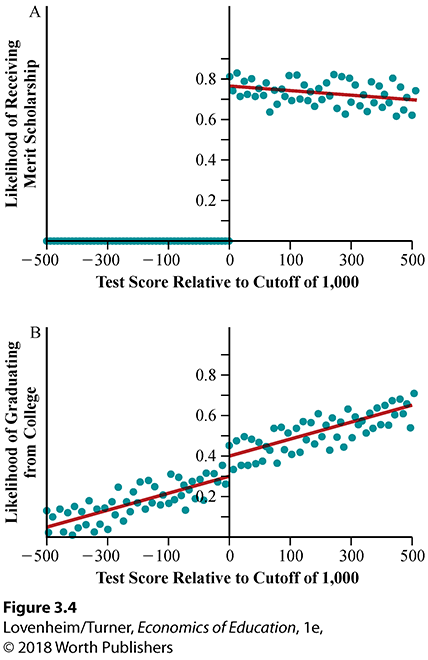
\includegraphics[width = 2.15in]{turner1e_fig_03_04.png}
   		 \end{figure}
	\end{column}
	\begin{column}{0.48\textwidth}
		\begin{itemize}[<+->]
			\item In Figure A, we see there is a 75 percentage point difference in the likelihood of winning a merit scholarship at a test score cutoff (fuzzy cutoff) \bigskip
			\item We can use this fuzzy cutoff to estimate the effect of merit aid on graduating college
		\end{itemize}
		
	\end{column}
\end{columns}

\end{frame}


\begin{frame}
\begin{columns}
	\begin{column}{0.48\textwidth}
  		  \begin{figure}[h]
   			 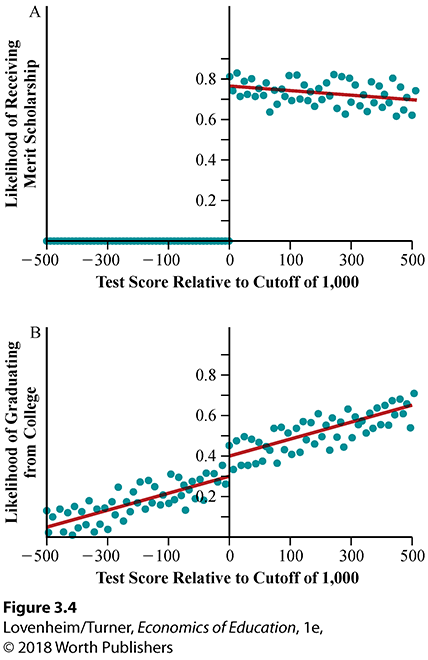
\includegraphics[width = 2.15in]{turner1e_fig_03_04.png}
   		 \end{figure}
	\end{column}
	\begin{column}{0.48\textwidth}
		\begin{itemize}[<+->]
			\item In a fuzzy framework, we divide the difference in outcomes at the threshold (10 percentage point increase in graduating from college (or .1)) by the difference in the likelihood of treatment (75 percentage points (or .75)) \medskip
			\item Here we find a 13.3 percentage point increase in the likelihood of graduating from college due to merit based financial aid
		\end{itemize}
		
	\end{column}
\end{columns}

\end{frame}












\end{document}




